%% Copernicus Publications Manuscript Preparation Template for LaTeX Submissions
%% ---------------------------------
%% This template should be used for copernicus.cls
%% The class file and some style files are bundled in the Copernicus Latex Package, which can be downloaded from the different journal webpages.
%% For further assistance please contact Copernicus Publications at: production@copernicus.org
%% https://publications.copernicus.org/for_authors/manuscript_preparation.html


%% Please use the following documentclass and journal abbreviations for discussion papers and final revised papers.

%% 2-column papers and discussion papers
\documentclass[essd, manuscript]{copernicus}

%% \usepackage commands included in the copernicus.cls:
%\usepackage[german, english]{babel}
%\usepackage{tabularx}
%\usepackage{cancel}
%\usepackage{multirow}
%\usepackage{supertabular}
%\usepackage{algorithmic}
%\usepackage{algorithm}
%\usepackage{amsthm}
%\usepackage{float}
%\usepackage{subfig}
%\usepackage{rotating}
\usepackage[ruled,vlined]{algorithm2e}

\begin{document}

\title{Decomposition of multispectral Sentinel-2 time series using neural networks for enhanced missing data imputation and compression.}


% \Author[affil]{given_name}{surname}

\Author[1]{Pablo R.}{Larraondo}
\Author[1]{Albert I. J. M.}{van Dijk}
%\Author[1]{Marta}{Yebra}

\affil[1]{Fenner School of Environment and Society. Australian National University. Canberra, Australia}

%% The [] brackets identify the author with the corresponding affiliation. 1, 2, 3, etc. should be inserted.

%% If an author is deceased, please add a further affiliation and mark the respective author name(s) with a dagger, e.g. "\Author[2,$\dag$]{Anton}{Aman}" with the affiliations "\affil[2]{University of ...}" and "\affil[$\dag$]{deceased, 1 July 2019}"


\correspondence{Pablo R. Larraondo (pablo.larraondo@anu.edu.au)}

\runningtitle{TEXT}

\runningauthor{TEXT}

\received{}
\pubdiscuss{} %% only important for two-stage journals
\revised{}
\accepted{}
\published{}

%% These dates will be inserted by Copernicus Publications during the typesetting process.

\firstpage{1}

\maketitle

\begin{abstract}
TEXT
\end{abstract}

\copyrightstatement{TEXT}

\introduction  %% \introduction[modified heading if necessary]

Remote sensing provides valuable information about the Earth with an increasing level of detail in the spatial, spectral and temporal domains. Due to the size of current remote sensing collections, processing the data requires accessing large amounts of storage and computing resources, making this task difficult and expensive. In the case of studying land processes, only the reflectance component coming from the Earth's surface is used, and all other effects originating in the atmosphere, such as clouds or shadows, can be considered noise contaminating the land's signal. Changes in the land typically happen at lower temporal scales than those in the atmosphere, which suggests that the land dynamics can be described a much lower dimensional space than the original data. This idea leads to the exploration of methodologies that exploit the inherent redundancies in the data and find efficient representations, able to capture the variability in the signal coming just from the land.

From an algebraic perspective, we can say that there exists a low-rank representation of the Earth's surface signal that is able to capture most of the variability in the original signal. Finding this low-rank representation is the objective of Principal Component Analysis (PCA). The use of PCA in remote sensing has been known for many years, and it has been extensively explored in the context of noise filtering and the compression of satellite images.

One of the limitations of PCA is its inability to work with missing values. As discussed before, remote sensing images representing the land surface, are often contaminated with atmospheric signals that need to be filtered, creating gaps of missing data in the images. There are different approaches for removing missing values for applying PCA, such as temporal aggregation of pixels, assigning fixed values to the missing data, or using different forms of interpolation through space or time. Therefore, the resulting decomposition performed by the PCA would depend on the process used to estimate values for the missing data. Regardless of the quality of the method employed for removing the missing values, artificial, non-observed values are introduced in the original signal, leading to errors and biases in the resulting decomposition.

PCA calculates the principal components of a matrix as the eigenvectors of its correlation matrix. This implies that principal components constitute an orthogonal basis for reconstructing the original matrix. This orthogonality constraint ensures that the information expressed by each component is unique and independent from the others. However, from an optimisation point of view, orthogonality makes the decomposition problem to be non-convex. Removing the orthogonality constraint ensures the decomposition is convex, which allows applying common optimisation techniques, such as gradient descent, to find valid decompositions of the original data. This idea of relaxing PCA constraints has been already proposed \citep{udell2014generalized} presenting a framework for generalising low-rank models.

Building upon the previous framework, this work explores how neural networks can be used to find efficient decompositions of remote sensing time series data. We evaluate the accuracy and performance of the proposed methodology comparing its results to classical PCA. Considering that the proposed methodology can naturally deal with missing values, we evaluate the quality of the resulting imputed data and compare it to other forms of pixel interpolation through time, a common approach used for applying PCA. The experiments are performed using temporal series of Sentinel-2 data over a region in Australia.


\section{Data}

The Copernicus Sentinel-2 mission \citep{drusch2012sentinel} is a constellation of two polar-orbiting satellites Sentinel-2A and Sentinel-2B launched on the 23th of June 2015 and the 7th of March 2017, respectively. These satellites are placed in the same sun-synchronous orbit and scan the Earth with a combined revisit period of 5 days and spatial resolutions that range between 10 and 60 metres. Digital Earth Australia (DEA) \citep{dhu2017digital} is a platform that contains Sentinel-2 data for Australia. DEA facilitates access and enhances quality of the data by adding further processing, such as correction for atmospheric and terrain effects. DEA data is stored using the Albers equal area projection for ensuring pixel size remains constant independent of its location.

To run the experiments in this work we extracted from DEA a 7000 km\textsuperscript{2} area around the Australian Capital Territory region comprising the years 2018 and 2019. Spectrally, we chose a subset of seven bands: three in the visible channels, two in the near infra-red and two in the short wave infrared, corresponding to bands (2, 3, 4, 8, 8a, 11, 12) in the original dataset. Bands 8a, 11, and 12 have nominal resolutions of 20 metres and were upsampled into 10 metres using nearest neighbour to achieve a homogeneous resolution across all bands.

The data was then split using regular tiles of 4 square kilometers each comprising the whole temporal extent. Figure \ref{dataset} shows a map of the region and the extent of each tile within a 16 by 23 grid. Using a contiguous region, as opposed to sparse isolated tiles, ensures the dataset contains a fair mix of tiles that are fully and partially filled with image data, due to random intersections with the original Sentinel-2 scenes. The objective is to consider a dataset that is manageable to carry out the experiments but that is representative of the original data. The results of this work should be easily reproduced for any other location.

\begin{figure}%
    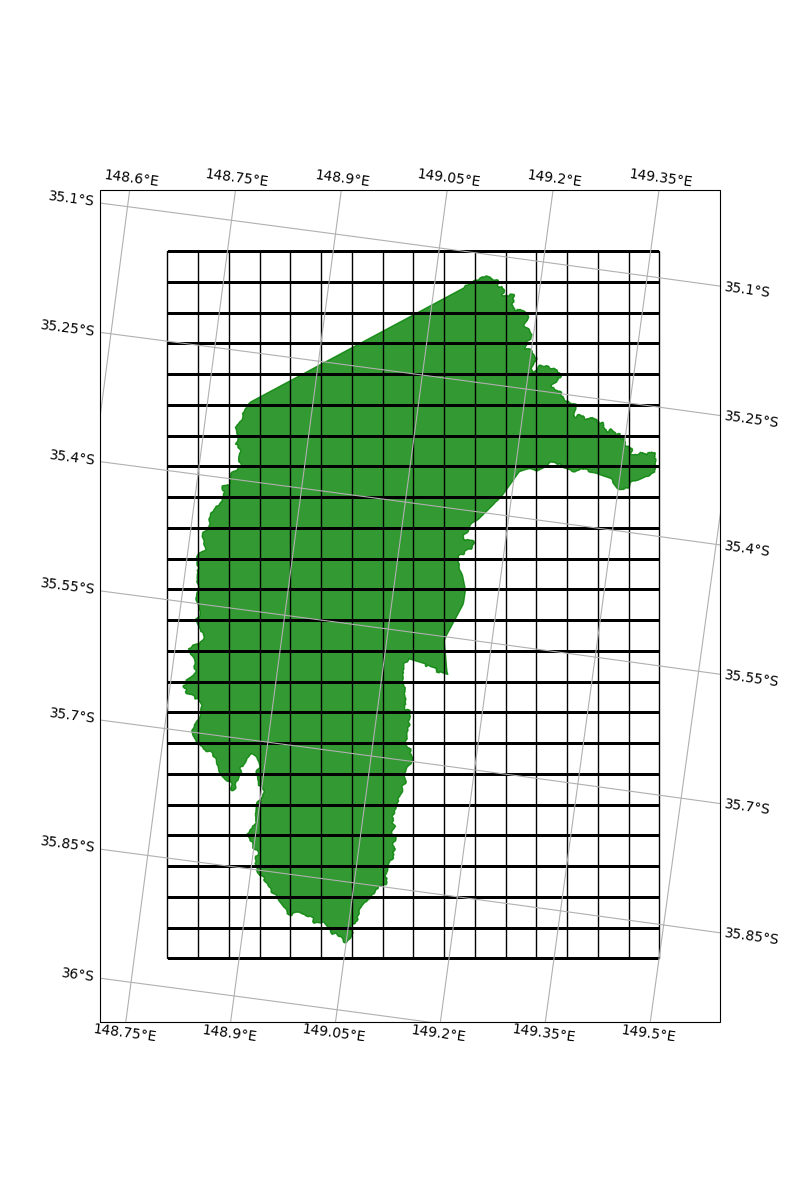
\includegraphics[width=10cm]{fig1.png}
    \caption{Region of the ACT with extents of the Sentinel 2 tiles.}%
    \label{dataset}%
\end{figure}

Each tile, as described previously, can be represented using a cube formed stacking 400 by 400 pixel images along the temporal dimension. In time, the number of images ranges between 85 and 130 depending on the position of the tile. The data was stored stacking each of the seven spectral bands in the same time dimension. Figure \ref{dataset_detail} represents the tile in the top-left corner in the dataset, with images corresponding to different dates stacked along the vertical dimension. On the left, the true colour composite is represented. On the right, the seven spectral bands are stacked together along the time dimension, as used in the experiments. 

\begin{figure}%
    {{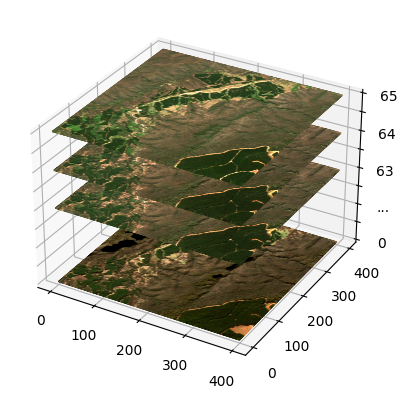
\includegraphics[width=4cm]{fig2a.png} }}%
    {{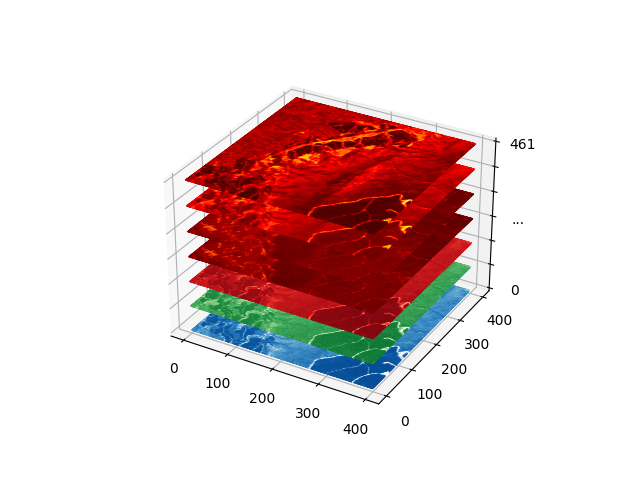
\includegraphics[width=4cm]{fig2b.png} }}%
    {{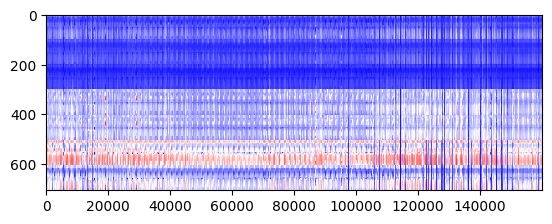
\includegraphics[width=8cm]{fig2c.png} }}%
    \caption{Tile corresponding to the top-left corner in the dataset (a) temporal stack of true colour images, (b) temporal stack of spectral images, (c) multi-spectral stack reshaped into 2-dimensional matrix}%
    \label{dataset_detail}%
\end{figure}

\subsection{Filtering clouds and shadows}
The atmosphere, standing between the satellite and the Earth's surface, modifies the spectral response coming from the ground. Clouds, haze, and other atmospheric meteors affect ground measurements and can be considered as noise contaminating the signal coming from the Earth. For our experiments, we want to capture the variability coming from the ground and then, we need to remove all other sources of variability in the data.

Several methodologies for removing clouds from Sentinel-2 images have been proposed \citep{louis2016sentinel,hagolle2017maja,qiu2019fmask}. These methodologies can be classified into single-date and multi-temporal algorithms \citep{}. For a comprehensive review and performance comparison of cloud detection methodologies, we refer readers to \citep{zhu2018cloud}. Multi-temporal algorithms are generally more accurate when compared to single-date ones, but have the inconvenient of being more difficult to implement and compute intensive.

In this work, we propose a new simple multitemporal methodology to detect pixels containing clouds and shadows. This methodology defines a series of dynamic thresholds used to determine if each pixel corresponds to either clear sky, cloud, or shadow categories. This methodology employs two Sentinel-2 spectral bands, blue (490 nm) and narrow nir (865 nm) and is easy to implement and efficient to run compared to other multitemporal methods \citep{frantz2015enhancing,zhu2018automatic}.

The proposed methodology assumes a 3-dimensional array of images stacked along time. 

Atmospheric processes normally have a much higher temporal variability than the ones occurring on the Earth's surface. Temporal based methods exploit this difference in the variability to detect outliers that can be attributed to atmospheric processes. Temporal based methods  


\section{Methodology and experimental design}

Principal Component Analysis (PCA) is a technique for reducing the dimensionality of datasets while maintaining as much of their original variance. PCA performs this dimensionality reduction by finding a new orthogonal basis where the original data is projected. The dataset is commonly represented by a matrix $M$ which is factorised into a product of two matrices of smaller size named matrix of principal components and coefficients. PCA of $M$ is generally computed through the singular value decomposition (SVD) of the covariance matrix $M^TM$. The resulting principal components of this process have the characteristic of being orthogonal to each other. The Eckart-Young theorem \citep{eckart1936approximation}, proves that this decomposition, truncated to the first $n$ factors, is the best rank-n approximation in the least squares sense, amongst all possible decompositions of $M$. 

Although PCA achieves the best factorisation of $M$, this solution is not unique and other methods can be employed to find alternative decompositions with the same error. In particular, we can relax the orthogonality constraint in PCA and use gradient descent optimisation to solve this problem. From an optimisation point of view, the relaxed non-orthogonal matrix factorisation problem can be formulated as:

$$
\arg\:\min_{AB} \mathbf{MSE}(M-AB)
$$

Where $\mathbf{MSE}$ stands for the mean square error and $A$ and $B$ are the factor matrices to optimise. The objective of this optimisation problem is to find the best $A$ and $B$ matrices whose product gives the best approximation of $M$.

In this work, we employ neural networks to solve this problem using gradient descent optimisation. The neural network to represent this problem can be constructed using two layers, where each of them represents one matrix or factor. The neural network is then trained to minimise the distance between the original matrix $M$ and the product of these two layers, denoted by matrices $A$ and $B$. As opposed to the common use of neural networks, we do not consider any non-linear activation functions, which means that we limit our exploration to purely linear models in this work. In PCA, we commonly refer to $A$ as the coefficients matrix and $B$ as the principal components matrix. Although the NN methodology generates different factorisations to PCA, we intentionally use the same terminology to refer to these factor matrices for establishing a link between both methodologies and improving clarity.

As described in the previous section, we consider $M$ to be the matrix containing the temporal series of satellite images, represented in Figure \ref{dataset_detail} c). We assume that the dynamics of the landscape, expressed through the evolution in time of the different spectral bands, can be expressed by a matrix $M'$, that has a significantly lower rank than the original matrix. This rank is determined by truncating the size of the decomposed matrices, or in terms of PCA decomposition, by limiting the number of principal components. As the number components is increased, the error in the factorisation is reduced, getting to zero when the number of components equals the rows (time dimension) of $M$. Figure \ref{explained_variance_evolution} represents the evolution of the explained variance in the recovered matrix $M'$ as the number of components is increased. To perform the experiments in this work, we fixed the number of components to 12, which gives a fair compromise between the quality of the recovered signal and the compression ratio. 

Figure \ref{factorisation} represents the reconstruction of the unbiased satellite observation matrix, $M$, as the product of two matrices, $A$ and $B$. Matrix $M$ in this figure contains 138 rows and 160000 columns, corresponding to the temporal dimension and number of pixels (400x400) respectively. In the shown decomposition, the number of components is truncated to 12. Matrix $B$ has size (12, 160000) corresponding to 12 principal components and the 400x400 spatial shape of the original tiles. Matrix $A$ represents the coefficients that multiply each of the principal components to recreate the temporal entries in the original matrix $M$. The number of columns of $A$ is the same as the rows of $B$, which determines the truncation performed in the factorisation. The level of truncation sets therefore a trade-off between the achieved accuracy of the reconstruction and the achieved compression ratio of the original matrix $M$. In this case, the compression ratio can be calculated considering the total size of the matrices on each side of the equality. The ratio $(138 \cdot 160000) / ((138 \cdot 12) + (12 \cdot 160000))$ tells us that the factors $A$ and $B$ are 84 times smaller than the initial matrix $M$. 

\begin{figure}%
    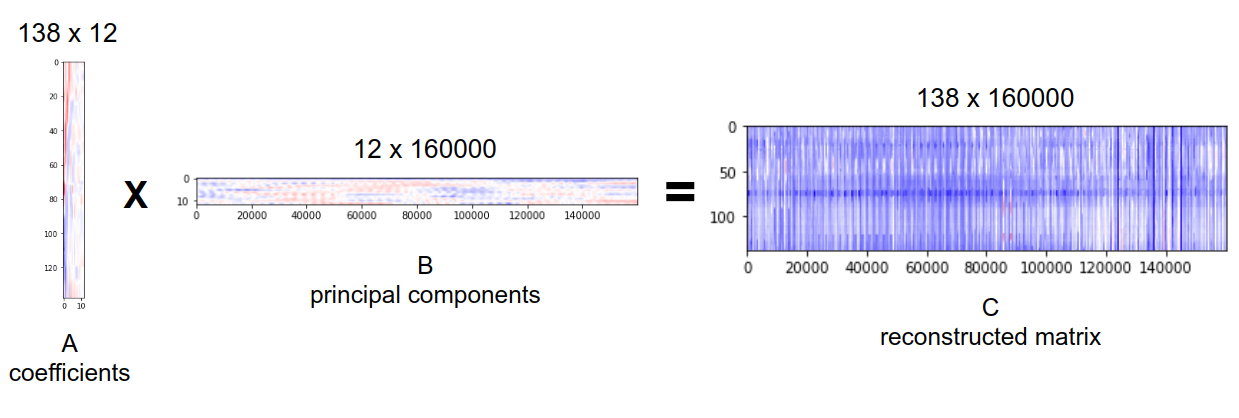
\includegraphics[width=10cm]{fig3.png}
	\caption{Reconstruction of the matrix of observations as the product of two factorised matrices, known as the matrix of coefficients (left) and principal components (right) in the case of PCA.}%
    \label{factorisation}%
\end{figure}


\begin{figure}%
    {{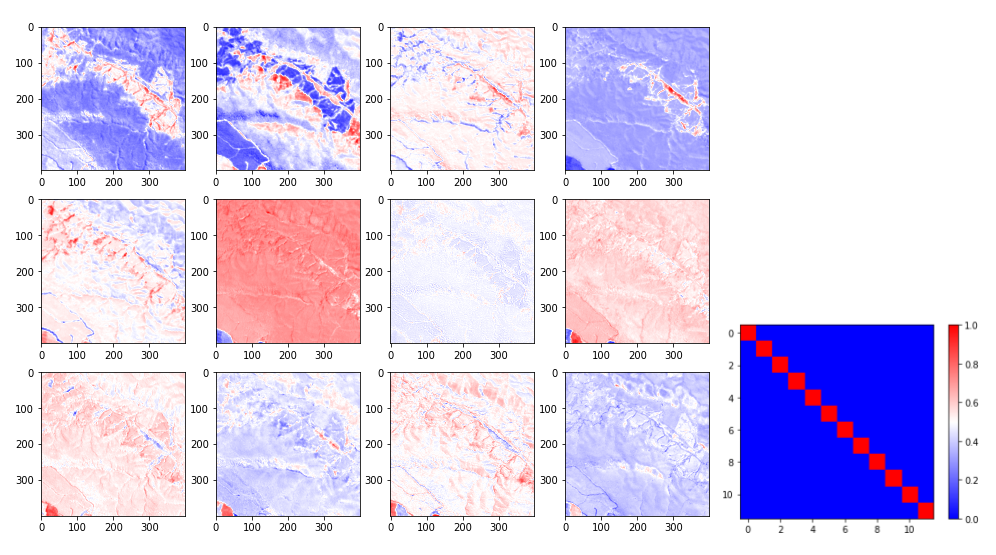
\includegraphics[width=8cm]{fig4a.png} }}%
    {{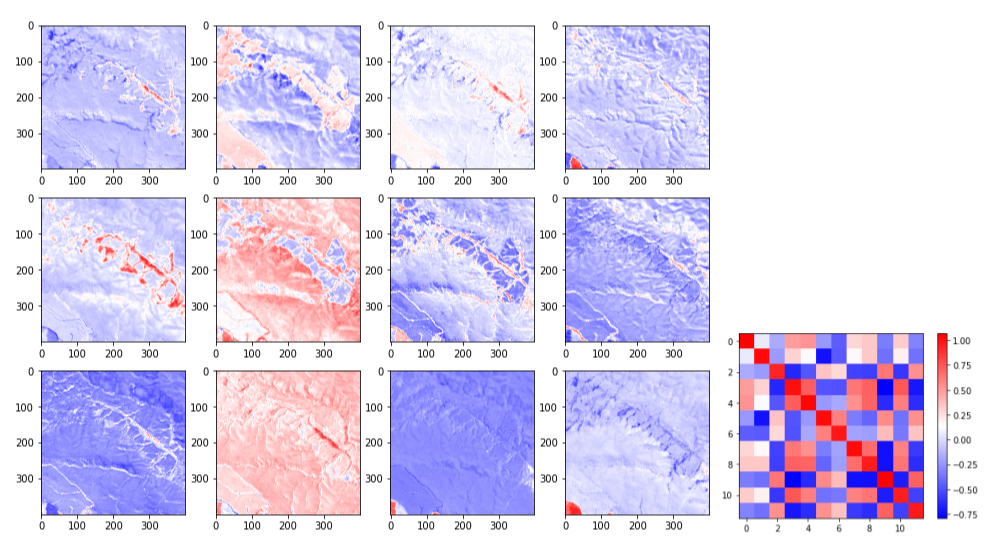
\includegraphics[width=8cm]{fig4b.png} }}%
	\caption{Representation of the 12 principal components matrix in Figure \ref{factorisation} as calculated by PCA (left) and the NN (right). Each component has been reshaped into the original 400x400 size of the original tiles.}%
    \label{pcs}%
\end{figure}

Figure \ref{pcs} represents the 12 principal components in matrix $B$ computed using PCA (left) and NN (right) reshaped into the original 400x400 size of the stack of images. The plots on the lower right show the product $B^TB$, which represents the inner products between each component. In the case of PCA, $B^TB$, shows entries equal to one along the main diagonal and zero everywhere else. This confirms that principal components resulting from PCA form an orthonormal basis. On the right, the $B^TB$ resulting from the NN factorisation, has heterogeneous values across the matrix, which means that the computed components are not orthogonal. Another difference between both methodologies is that the principal components computed with PCA are ordered by importance at explaining the variance in the original signal (from top-left to bottom-right) but not such ordering exists in the case of NN (this can be verified looking at the values of the coefficients matrix in each case). We note that as opposed to PCA, the decomposition achieved with the NN method is not unique and varies between runs. The order of the components (columns of $B$) and the magnitude of the elements in the matrices can vary and still generate the same product.

The following sections describe the two main contributions in this work and the proposed experiments used to evaluate them.

\subsection{Missing data imputation}

One of the limitations of PCA is its inability to deal with missing values. Consequently, it is a common practice to interpolate or assign pre-fixed values to any missing entries before applying PCA. In the case of NNs, the factorisation is performed minimising the mean squared difference between the initial matrix $M$, containing missing values, and the product of matrices $A$ and $B$, which is complete. The previous error can be computed masking out the positions with missing values in both matrices and optimise the network, so this error is minimised. The resulting decomposition generates a full matrix $M'$ with imputed missing values.

Using this methodology, the principal components and coefficients are adjusted to the regions with known values. The missing value imputation process extends the values of the principal components modulated by the learnt coefficients to the whole image. This process constitutes therefore a spatial interpolation methodology to interpolate missing values on individual temporal images. To assess the quality of the imputation methodology, we compare the results with interpolation of pixels along the temporal dimension.

The quality of the missing value imputation process is directly proportional to the number of principal components employed to factorise the matrix containing the observations. To perform a fair evaluation of the quality of this method, we compare it with the results of PCA on temporally interpolated data using the same number of components. To assess the differences between methodologies, we randomly masked 80x80 pixel patches with known values in the image stack as missing data. The new dataset, with the extra missing values, was then used to train our NN and also to perform PCA previously interpolating the missing values along the temporal dimension. Using the previous mask, the patches with initial missing data where isolated and compared with the original values in the observation matrix. 

Figure \ref{dataset_versions} represents the masking process performed to evaluate the missing data imputation process using one sample in the time series stack of images. On the first row, we represent one image randomly masked with a 80x80 patch. These masked data are factorised resulting in a complete dataset with no missing values. The masked regions are then isolated and its values compared with those in the original dataset.

\begin{figure}%
    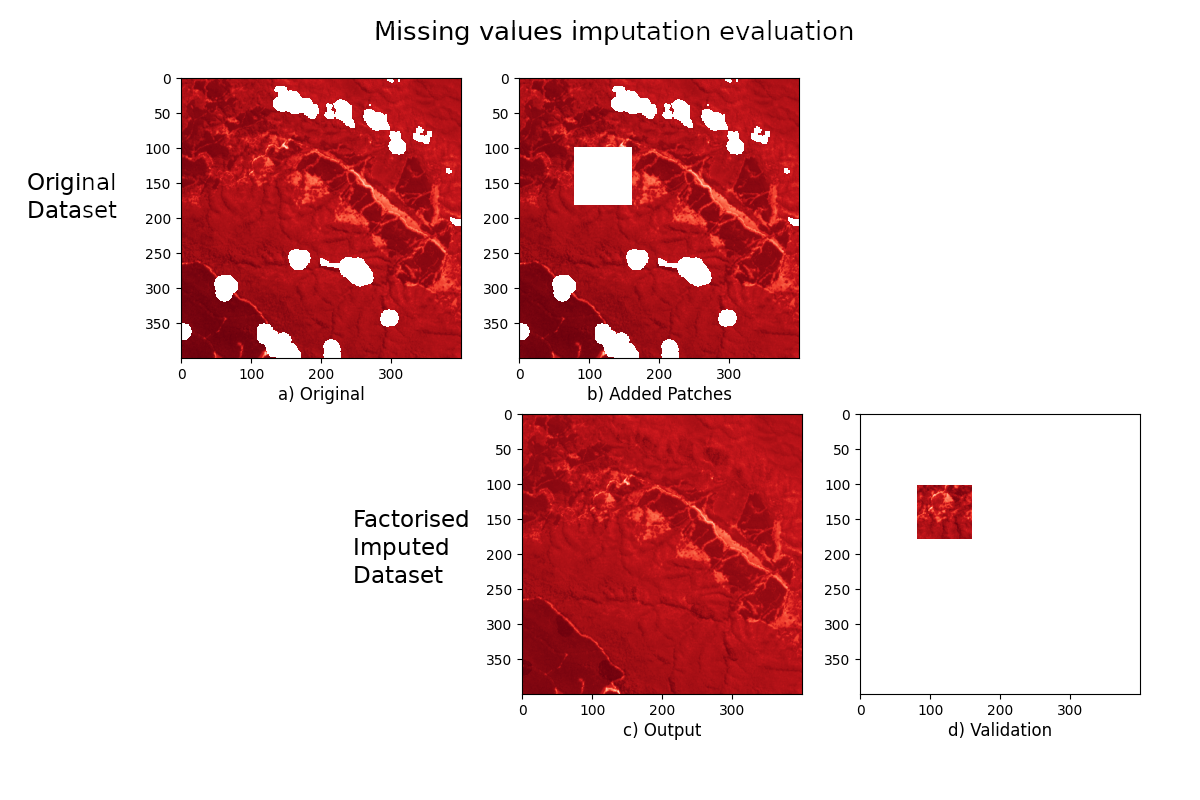
\includegraphics[width=14cm]{fig5.png}
    \caption{Masking process for comparing missing data imputation accuracy.}%
    \label{dataset_versions}%
\end{figure}

The comparison between the NN imputation and the pre-interpolated PCA is evaluated using the mean squared error on the randomly selected patches.

\subsection{Multispectral data compression}

Multispectral satellite imagery is able to reveal the Earth's surface composition through well-known reflectance patterns across the spectral bands. Although each of the multispectral bands contains unique information, the general spatial structure of a region is more or less equally represented across the electromagnetic spectrum. This spatial similarity between spectral bands can be exploited to create more compact representations of the data. In this section, we explore the possibility of learning principal component representations shared between spectral bands as opposed to decomposing each spectral band separately.

Using a naive approach, we can stack all the spectral bands and form a matrix similar to $M$, as represented in Figure \ref{factorisation}, but containing $n$ times more rows, where $n$ is the number of spectral bands. The difference with the previous experiments is that the new extracted principal components would be shared between the spectral bands. The benefit of this approach is that the resulting decomposition is $n$ times more efficient in size when compared to performing the decomposition on individual bands. The drawback, on the other hand, is that the quality of the reconstructed matrix containing all bands at once is not as good as decomposing each band individually. To identify the level of redundancy shared between spectral bands, we designed an experiment that compares the number of components used in each approach for a given error of the reconstructed matrix. 

One of the main benefits of using NNs to perform matrix decompositions is the possibility of exploring alternative architectures. The field of image analysis using NNs has recently experienced a rapid development due primarily to the use of deep convolutional neural networks (CNN). CNNs are a type of neural network that include convolutional operations in their layers. The convolution operations are normally performed across the spatial domain of images and are used to identify patterns between nearby pixels.

In this work, we propose a new NN architecture that extends the simple matrix factorisation including a convolutional layer. This architecture is able to factorise multispectral images with a significant improvement of accuracy when compared to the basic methodology. Figure \ref{factorisation_methods} shows a comparison between the basic factorisation architecture and the convolutional one. In both cases, the networks are trained using gradient descent to find the matrices represented on the left side of the figure. In the basic architecture, the NN minimises the difference between the matrix with the stacked observations and the product of the the principal components and factors matrices. The convolutional factorisation architecture introduces an extra element, the convolutional kernel. This kernel is a 4-dimensional tensor which is applied to the principal component tensor in its original 3-dimensional shape. This kernel performs a convolution operation on the tensor containing the principal components extending the number of principal components. 

\begin{figure}%
    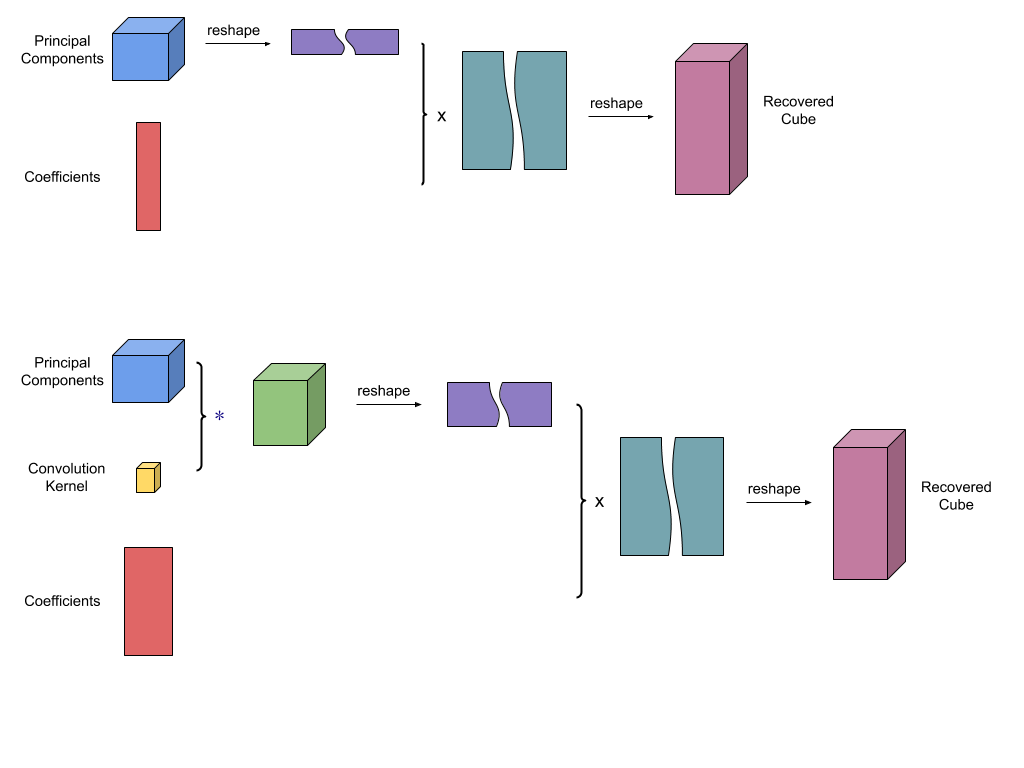
\includegraphics[width=14cm]{fig6.png}
    \caption{Comparison between the baseline and convolutional NN factorisation methodologies.}%
    \label{factorisation_methods}%
\end{figure}

In terms of the level of compression achieved by these factorisations, the matrix of principal components accounts for most of the space in the compressed versions. Using our example dataset, adding an extra principal component to the factorisation requires storing 160,000 (400x400) extra elements in the principal components matrix but only 138 (time steps) in the coefficients matrix. It is therefore in our interest to prioritise finding better representations of the principal components matrix. In this work, we propose the introduction of the convolution kernel as an indirect way of expanding the number of components in the principal components matrix. In the case of considering 12 principal components and a 5x5 convolutional kernel that doubles this number of components to 24, we would be adding a 4-dimensional tensor with size 5x5x12x24=7200, which is still significantly smaller than a single principal component. The idea is that by adding a small size component to the network, we are able to effectively expand the number of components in the factorisation.

In the next section, we present the results of the experiments that assess the missing data imputation and compression capabilities of the proposed methodologies. 


\section{Experimental results and discussion}

\subsection{Comparison of methodologies}
We start by showing a comparison between the PCA and NN factorisation methodologies for decomposing Sentinel-2 temporal series. Using the entire dataset, we applied the algorithm shown in Appendix A to remove clouds and shadows from the images. The missing values in the resulting single spectral band image stacks were then filled applying a linear interpolation to each pixel along the temporal dimension. The 368 tiles comprising the Australian Capital Territory were cleaned from atmospheric contamination and subsequently interpolated. These tiles, with no missing values, were then factorised using the PCA and NN methodologies using several levels of truncation. Table \ref{components_error} shows the mean reconstruction errors for each methodology and spectral band averaged across all the tiles in the dataset. 

\begin{table}
\centering
\begin{tabular}{|l|l|r|r|}
\toprule
\hline
             &    &   PCA MSE* &    NN MSE* \\
Band Name & Truncation &           &           \\
\midrule
\hline\hline
nbart\_blue & 8  &  0.854292 &  0.854301 \\
             & 12 &  0.854292 &  0.854301 \\
             & 16 &  0.854292 &  0.854301 \\
\hline
nbart\_green & 8  &  0.999367 &  0.999374 \\
             & 12 &  0.999367 &  0.999374 \\
             & 16 &  0.999367 &  0.999374 \\
\hline
nbart\_nir\_1 & 8  &  5.769267 &  5.769406 \\
             & 12 &  5.769267 &  5.769406 \\
             & 16 &  5.769267 &  5.769406 \\
\hline
nbart\_nir\_2 & 8  &  4.600799 &  4.600894 \\
             & 12 &  4.600799 &  4.600894 \\
             & 16 &  4.600799 &  4.600894 \\
\hline
nbart\_red & 8  &  2.165023 &  2.165069 \\
             & 12 &  2.165023 &  2.165069 \\
             & 16 &  2.165023 &  2.165069 \\
\hline
nbart\_swir\_2 & 8  &  6.402195 &  6.402738 \\
             & 12 &  6.402195 &  6.402738 \\
             & 16 &  6.402195 &  6.402738 \\
\hline
nbart\_swir\_3 & 8  &  5.655861 &  5.656370 \\
             & 12 &  5.655861 &  5.656370 \\
             & 16 &  5.655861 &  5.656370 \\
\bottomrule
\hline
\end{tabular}
\caption{MSE comparison of the reconstructed Sentinel-2 time series data using PCA and NN methodologies for different truncation levels. (* 1E-5)}
\footnote{* 1E5footnote text}
\label{components_error}
\end{table}

The errors in Table \ref{components_error} imply that the quality of the factorisations achieved with both methodologies are the same (up to numerical precision) across the range of considered truncations. This result also proves that the best decomposition (Eckart-Young theorem) estimated using PCA is not unique (or can be closely matched), when non-orthogonal basis are considered.

\subsection{Missing value imputation methodology assessment.}
In the previous experiment we showed the equivalence of PCA and NN factorisation methodologies using complete data, with no missing values. In this part, we evaluate the missing data imputation capabilities of the NN decomposition approach. The comparison is performed using regions of known data, which we intentionally assign to no data values. Following the method presented in section 3.1, each stack of images in the dataset was masked with 20 40x40 pixel patches of missing values randomly spread across the spatial and temporal dimensions. The resulting dataset was then factorised using the NN methodology with 12 principal components and its results compared to those of the PCA computed using the linearly interpolated version of the dataset using the same number of components. The mean squared error of each factorisation method was calculated considering the original known values in just the masked regions. Figure 

\begin{figure}
    \includegraphics[width=10cm]{fig7.png}
    \caption{Bar plot showing the MSE error of the imputed values Comparison between the basic the convolutional factorisation methodologies.}%
    \label{multispectral_cmp}%
\end{figure}

The NN factorisation methodology has a double function, it imputes missing values and also reduces the rank of the input signal. As the number of components or the level of truncation is increased, the quality of the missing data imputation process is increased. To perform a fair comparison, this methodology needs to be compared with other methods that generate the same level of truncation to the data. In this case the comparison is made with the PCA decomposition of the linear temporal interpolation of the data using the same number of components. 

\subsection{Multispectral convolution compression methodology assessment.}
In the previous experiments, only one spectral band has been used for evaluating the decomposition methodologies. As mentioned in the previous section, high-level spatial features are commonly shared across spectral bands and this redundancy in the spectral bands allows for aggregating spectral bands and decomposing the multispectral data. The resulting principal components in this case are shared between the spectral bands and the reconstruction error varies between bands. Certain types of soil, vegetation or moisture conditions are represented very differently by spectral bands and these unique features are not well represented by the principal components. To assess the quality of the multispectral decomposition and the variability of the reconstruction error for the different bands, we compare the MSE of the reconstructed images for the multispectral and single band decompositions using the Sentinel-2 dataset. 

In the next experiment, we assess the decompostion NN architecture that includes the convolutional layer, as shown in Figure \ref{factorisation_methods}. To run the experiment we chose a 5x5 kernel that expanded the number of principal components from 12 to 24. The elements of this convolution kernel were set during the training process of the network to identify patterns and relationships between the input spectral bands. Using a similar representation as previously, Figure \ref{factorisation_methods} compares the reconstruction error of the basic and convolutional NN architectures fixing the truncation to 12 components in both cases. Note that the 12 components are internally transformed into 24 by the convolution kernel in the second case.

\begin{figure}
    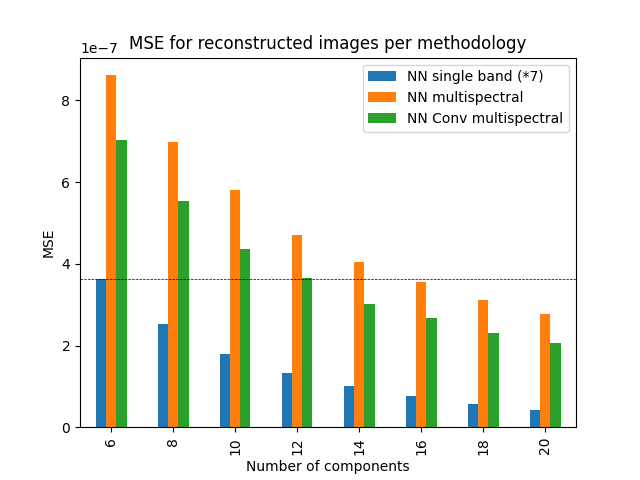
\includegraphics[width=10cm]{fig8.png}
    \caption{Comparison between the basic the convolutional factorisation methodologies.}%
    \label{compression_cmp}%
\end{figure}


In terms of compression ratio, we evaluated the storage efficiency of each of these methodologies at different truncation levels. Figure \ref{compression_cmp} represents the MSE of the reconstructed images for the basic and convolutional NN architectures and the bands compressed separately. 
Figure \ref{multispectral_cmp} shows the MSE of the reconstructed images for each method. The red bar represents the error of the multispectral decomposition using 12 components, the green bar represents the error of the decomposition of the single band using 12 components and the blue bar, shown as reference, represents the error of the multispectral decomposition using 84 components (12 components per spectral band). These results show that the multispectral decomposition generates more efficient representations when compared to factorising each band separately. 


\conclusions  %% \conclusions[modified heading if necessary]
In this paper, we evaluated the application of NNs to decompose remote sensing data in the presence of missing values as an alternative to other interpolation methods. The methodology was evaluated using Sentinel-2 time series data for the Australian Capital Territory region. The NN-based methodology achieved better compression ratios and accuracy at interpolating missing values when compared to PCA. We demonstrate that relaxing the orthogonality constraints of PCA improves compression for time series of satellite multispectral data.

Additional studies are planned to evaluate the effect of non-linearities and convolution operations in the network. Another avenue for exploration is the introduction of constraints that lead to sparsity to enhance compression and improve interpretability of the results. 

The cloud and shadow filtering step was performed as a pre-processing step in this work. The quality of this step has a great influence on the quality of the results. Pixels with non-detected clouds increase variance in the temporal series and tend to be represented in the decomposed principal components degrading the quality of the results. Ideally, this pre-processing step could be avoided by designing a neural network that is able to decompose input signals contaminated by noise. We are currently exploring the possibility of building this end-to-end network.

%% The following commands are for the statements about the availability of data sets and/or software code corresponding to the manuscript.
%% It is strongly recommended to make use of these sections in case data sets and/or software code have been part of your research the article is based on.

%\codeavailability{TEXT} %% use this section when having only software code available


%\dataavailability{TEXT} %% use this section when having only data sets available


\codedataavailability{} 
%% use this section when having data sets and software code available
The code used to process the data and run the experiments in this paper is publicly available at: \\
\href{https://github.com/prl900/unet_him8_gpm}{https://github.com/prl900/unet\_him8\_gpm}. \\
Sentinel-2 Surface Reflectance NBART data used in the experiments comes from Geoscience Australia's Digital Earth Platform \href{https://cmi.ga.gov.au/data-products/dea/190/dea-surface-reflectance-nbart-sentinel-2-msi}{https://cmi.ga.gov.au/data-products/dea/190/dea-surface-reflectance-nbart-sentinel-2-msi}. 

%\sampleavailability{TEXT} %% use this section when having geoscientific samples available

%\videosupplement{} %% use this section when having video supplements available

\appendix
\section{Cloud \& shadow masking algorithm} %% Appendix A

The cloud and shadow filtering process followed in this work can be described using two steps. In a first step, bright pixels can be removed using the blue channel and then two rolling median through time are calculated for the blue and narrow near-infrared channels. Remaining missing data are filled using nearest neighbour interpolation through time. The result of this step are two arrays of the same dimensions as the initial ones, where pixels with high reflectance values on the blue channel have been removed and the values of the pixels are smooth in time using a temporal median filter. The purpose of this step is to have a clean stack of images that captures long-term trends in the signal to be used as reference in the next step.

Useful??kk? Changes in reflectance values or local textures that are separable from changes caused by other factors such as differences in atmospheric conditions, illumination and viewing angles, and soil moisture \citep{deng2008pca}.

\begin{algorithm}[H]
\SetAlgoLined
 \Comment{\#1. Load Sentinel-2 data from spatial and temporal extents}\\
 blue = load(ds:sentinel2, band:blue, x:[xstart,xend], y:[ystart,yend],time:[tstart,tend])\\
 nnir = load(ds:sentinel2, band:narrow\_nir, x:[xstart,xend], y:[ystart,yend],time:[tstart,tend])\\
 \\
 \Comment{\#2. Assign pixels with blue reflectances exceeding lower quartile value by more than 10\% to NaN.}\\
 blue[(blue - blue.percentile(0.25)) $>$ 0.1] = NaN\\
 nnir[(blue - blue.percentile(0.25)) $>$ 0.1] = NaN\\
 \\
 \Comment{\#3. Entirely wipe images with more than 66\% missing pixels}\\
 blue[(blue.count\_nan(axis=1,2) $>$ width*hight*0.66] = NaN\\
 nnir[(nnir.count\_nan(axis=1,2) $>$ width*hight*0.66] = NaN\\
 \\
 \Comment{\#4. Calculate rolling median along time dimension and interpolate missing values}\\
 blue\_median = blue.rolling\_median(window\_size=7).interpolate(method=nearest)\\
 nnir\_median = nnir.rolling\_median(window\_size=7).interpolate(method=nearest)\\
 \caption{Step 1: rolling median calculation.}
\end{algorithm}

The second step uses these rolling median stacks to detect anomalies in the original stacks. 

\begin{algorithm}[H]
\SetAlgoLined
 \Comment{\#1. Load Sentinel-2 data from spatial and temporal extents}\\
 blue = load(ds:sentinel2, band:blue, x:[xstart,xend], y:[ystart,yend],time:[tstart,tend])\\
 nnir = load(ds:sentinel2, band:narrow\_nir, x:[xstart,xend], y:[ystart,yend],time:[tstart,tend])\\
 
 \Comment{\#2. Calculate rolling medians using the previous algorithm}\\
 blue\_median = step1(blue)\\
 nnir\_median = step1(nnir)\\
 
 \Comment{\#3. Calculate mask using deviations from the rolling median values}\\
 blue\_mask = (blue - blue\_median) $>$ 0.01 + blue\_median/2\\
 nnir\_mask = (nnir - nnir\_median) $<$ -0.06 + nnir\_median/16\\
 mask = blue\_mask $\parallel$ nnir\_mask\\
 \\
 \Comment{\#4. Remove small clusters and dilate remaining ones}\\
 mask = remove\_small\_objects(mask, min\_size=9)\\
 mask = dilate(mask, disk=9)\\
 \caption{Step 2: Mask calculation using deviations from the blue and narrow nir rolling means.}
\end{algorithm}

These algorithms have been specified in pseudo-code using a notation similar to Python's Numpy and Xarray libraries. We refer readers to \href{https://github.com/prl900/unet_him8_gpm}{https://github.com/prl900/unet\_him8\_gpm} for a working implementation of this algorithm.

%\subsection{}     %% Appendix A1, A2, etc.


\noappendix       %% use this to mark the end of the appendix section

%% Regarding figures and tables in appendices, the following two options are possible depending on your general handling of figures and tables in the manuscript environment:

%% Option 1: If you sorted all figures and tables into the sections of the text, please also sort the appendix figures and appendix tables into the respective appendix sections.
%% They will be correctly named automatically.

%% Option 2: If you put all figures after the reference list, please insert appendix tables and figures after the normal tables and figures.
%% To rename them correctly to A1, A2, etc., please add the following commands in front of them:

\appendixfigures  %% needs to be added in front of appendix figures

\appendixtables   %% needs to be added in front of appendix tables

%% Please add \clearpage between each table and/or figure. Further guidelines on figures and tables can be found below.



%\authorcontribution{TEXT} %% this section is mandatory

%\competinginterests{TEXT} %% this section is mandatory even if you declare that no competing interests are present

%\disclaimer{TEXT} %% optional section

\begin{acknowledgements}
Re-emergence or ANU-WALD bushfire centre? Ask Marta
We gratefully acknowledge the support of NVIDIA Corporation with the donation of the Titan Xp GPU used in this research.
\end{acknowledgements}

\bibliographystyle{copernicus}
\bibliography{refs.bib}

\end{document}
